\documentclass[]{article}
\usepackage{lmodern}
\usepackage{graphicx}
\usepackage{caption}
\usepackage{subcaption}
\usepackage{adjustbox}
\usepackage{amssymb,amsmath}
\usepackage{ifxetex,ifluatex}
\usepackage{listings}
\usepackage[T1]{fontenc}
\usepackage[utf8]{inputenc}
\usepackage{microtype}
\usepackage[margin=1in]{geometry}
\usepackage{hyperref}
\usepackage{framed}
\usepackage{grffile}
\makeatletter
\def\maxwidth{\ifdim\Gin@nat@width>\linewidth\linewidth\else\Gin@nat@width\fi}
\def\maxheight{\ifdim\Gin@nat@height>\textheight\textheight\else\Gin@nat@height\fi}
\makeatother
% Scale images if necessary, so that they will not overflow the page
% margins by default, and it is still possible to overwrite the defaults
% using explicit options in \includegraphics[width, height, ...]{}
\setkeys{Gin}{width=\maxwidth,height=\maxheight,keepaspectratio}
\setlength{\parindent}{0pt}
\setlength{\parskip}{6pt plus 2pt minus 1pt}
\setlength{\emergencystretch}{3em}  % prevent overfull lines
\providecommand{\tightlist}{%
  \setlength{\itemsep}{0pt}\setlength{\parskip}{0pt}}

%%% Change title format to be more compact
\usepackage{titling}

% Create subtitle command for use in maketitle
\newcommand{\subtitle}[1]{
  \posttitle{
    \begin{center}\large#1\end{center}
    }
}

\setlength{\droptitle}{-2em}
  \title{MSAN 601 - Homework 3}
  \pretitle{\vspace{\droptitle}\centering\huge}
  \posttitle{\par}
  \author{Andre Guimaraes Duarte}
  \preauthor{\centering\large\emph}
  \postauthor{\par}
  \predate{\centering\large\emph}
  \postdate{\par}
  \date{September 19, 2016}
  
% Redefines (sub)paragraphs to behave more like paragraphs
\ifx\paragraph\undefined\else
\let\oldparagraph\paragraph
\renewcommand{\paragraph}[1]{\oldparagraph{#1}\mbox{}}
\fi
\ifx\subparagraph\undefined\else
\let\oldsubparagraph\subparagraph
\renewcommand{\subparagraph}[1]{\oldsubparagraph{#1}\mbox{}}
\fi

\usepackage{color}
\usepackage{siunitx}

%%%%%%%%%%%%%%%%%%%%%%%%%%%%%%%%%%%%%%%%%%%%%%%%%%%%%%%%%%%%%%%%%%%%%%%%%%%%%%%%%%%%%%%%%%%%%%%%%%%%%%%%%%%%%%%%%%%%%%%
\begin{document}
\maketitle

\paragraph{\Large Question 1}\normalsize

\begin{table}[!ht]
\centering
\caption{Summary of results for \texttt{Transact} data.}
\begin{tabular}{|c|c|c|c|}
\hline
$Y = \beta_{01} + \beta_{11} t_1 + \beta_{21} t_2$ &
$Y = \beta_{02} + \beta_{32} a + \beta_{42} d$ &
$Y = \beta_{03} + \beta_{23} t_2 + \beta_{43} d$ &
$Y = \beta_{04} + \beta_{14} t_1 + \beta_{24} t_2 + \beta_{34} a + \beta_{44} d$ \\
\hline
$b_{01} = 144.36944$ & $b_{02} = 144.3694$ & $b_{03} = 144.3694$ & $b_{04} = 144.36944$\\
$b_{11} = 5.46206$ & $b_{32} = 7.4699$ & $b_{23} = 7.4699$ & $b_{14} = 5.46206$\\
$b_{21} = 2.03455$ & $b_{42} = 1.7138$ & $b_{43} = 5.4621$ & $b_{24} = 2.03455$\\
 &  &  & $b_{34} = \texttt{NA}$\\
 &  &  & $b_{44} = \texttt{NA}$\\
\hline

\end{tabular}
\label{q1}
\end{table}


a) As we can see from Table \ref{q1}, the coefficient estimates $b_{34}$ and $b_{44}$ for $\beta_{34}$ and $\beta_{44}$ are labeled as \texttt{NA}. Indeed, the variables corresponding to these coefficients are $a$ and $d$, which are linear combinations of $t_1$ and $t_2$, that are already in the model. Consequently, matrix $X$ is no longer full-rank, and $X'X$ is not invertible (reminder: $X'X$ needs to be invertible to calculate $\hat{Y} = HY$, where $H = X(X'X)^{-1}X'$).

b) From Table \ref{q1}, we can see that $\beta_{0i}$ is the same for all four models. In addition, the F-statistic is the same (1289 on 2 and 258 degrees of freedom), as well as $R^2$ ($0.9091$) and $R^2_a$ ($0.9083$). This is true even for model (4). Indeed, since $a$ and $d$ are linear combinations of the other two variables, they are not included in the final model.

In addition, we can see that models (1) and (4) have the same coefficients, and are in fact the same model. In (2) and (3), we get $\beta_{32} = \beta_{23}$, but $\beta_{42} \neq \beta_{43}$.

c) We can see in Table \ref{q1} that the estimate for $t_2$ is different in (1) and (3). This is because the second regressor in each model is not the same ($t_1$ in (1) and $d$ in (3)). The impact of $t_2$ when $t_1$ is in the model is different from the impact of $t_2$ when  $d$ is in the model.

\paragraph{\Large Question 2}\normalsize

a) Here, we are modeling the variation of the log of \texttt{fertility} (the number of children per woman) as a linear function of \texttt{pctUrban} (the percent urban). With \texttt{R}, we get

$\text{log(fertility)} = 1.500963 - 0.010163*\text{pctUrban}$.

An increase in one unit in \texttt{pctUrban} (an additional percent in urban population) leads to an expected decrease in $0.010163$ units of the log of \texttt{fertility}. Since this is hard to interpret, let's convert the equation to get rid of the log. We get

\begin{tabular}{ccl}
$\text{fertility}$ & $=$ & $\exp{(1.500963 - 0.010163*\text{pctUrban})}$\\
                   & $=$ & $\exp{(1.500963)} \times \exp{(-0.010163*\text{pctUrban})}$
\end{tabular}

Therefore, an increase in 25 percent in urban population is written as

\begin{tabular}{ccl}
$\exp{(1.500963)} \times (1.25 \times \text{pctUrban})^{-0.010163}$ & $=$ &  $\exp{(1.500963)} \times 1.25^{-0.010163} \times \text{pctUrban}^{-0.010163}$\\
                   & $=$ & $0.9977348 \times \exp{(1.500963)} \times \text{pctUrban}^{-0.010163}$\\
                   & $=$ & $0.9977348 \times \text{fertility}$
\end{tabular}

As can be seen, this leads to a decrease in $1-0.9977348 = 0.0022652 = 0.22652\%$ in fertility.

b) We now have the following model

$\text{log(fertility)} = 3.50736 -0.06544*\text{log(ppgdp)} -0.02824*\text{lifeExpF}$.

We can re-write this equation to remove the logarithms:

\begin{tabular}{ccl}
$\text{fertility}$ & $=$ & $\exp{(3.50736 -0.06544*\text{log(ppgdp)} -0.02824*\text{lifeExpF})}$\\
 & $=$ & $\exp{(3.50736)} \times \exp{(-0.06544*\text{log(ppgdp)}) \times \exp{(-0.02824*\text{lifeExpF})}}$\\
 & $=$ & $\exp{(3.50736)} \times \text{ppgdp}^{-0.06544} \times \exp{(-0.02824*\text{lifeExpF})}$
\end{tabular}

A $25\%$ increase in \texttt{ppgdp} leads to the following equation:

\begin{tabular}{rl}
& $\exp{(3.50736)} \times (1.25 * \text{ppgdp})^{-0.06544} \times \exp{(-0.02824*\text{lifeExpF})}$ \\
$=$ & $\exp{(3.50736)} \times (1.25)^{-0.06544} \times \text{ppgdp}^{-0.06544} \times \exp{(-0.02824*\text{lifeExpF})}$\\
$=$ & $0.9855036 \times \exp{(3.50736)} \times \text{ppgdp}^{-0.06544} \times \exp{(-0.02824*\text{lifeExpF})}$\\
$=$ & $0.9855036 \times \text{fertility}$
\end{tabular}

As can be seen, this leads to a decrease in $1-0.9855036 = 0.0144964 = 1.44964\%$ in fertility.

\paragraph{\Large Question 3}\normalsize

a) Using \texttt{R}, we first have a look at the scatterplot for the data, and look at the correlations using \texttt{pairs} and \texttt{cor}. The scatterplot is shown in Figure \ref{fig3}, and the correlation matrix is shown in Table \ref{q3}. These results show us that the most likely candidate for an explanatory variable is $X2$.

\begin{figure}[!ht]
\centering
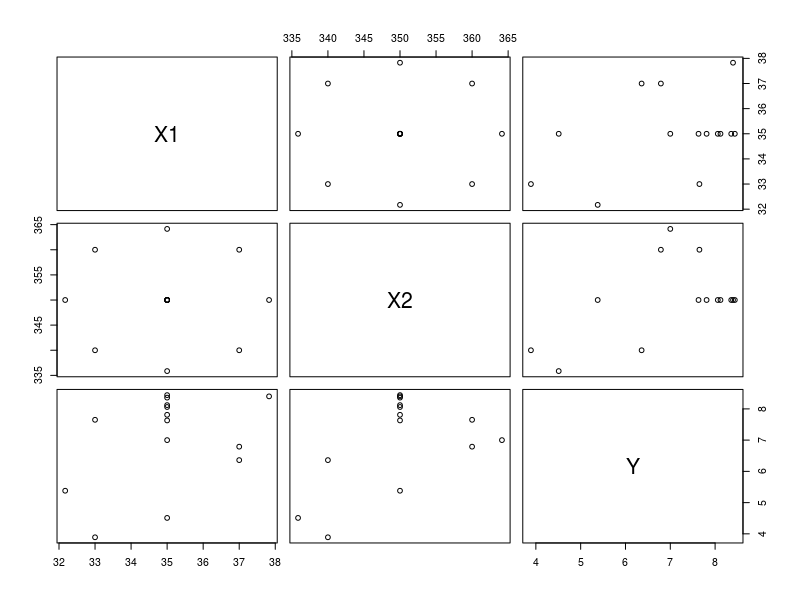
\includegraphics[width=\textwidth]{cakespairs.png}
\caption{Pairs plot of \texttt{cakes} data.}
\label{fig3}
\end{figure}

\begin{table}[!ht]
\centering
\caption{Correlation matrix for \texttt{cakes} data.}
\begin{tabular}{c|c|c|c|}
    &       Y      &       X1     &       X2       \\
\hline
 Y  &  1.00000000  &              &                \\
 X1 &  0.3882796   &  1.00000000  &                \\
 X2 &  0.5091336   &  0.0000000   &   1.00000000   \\
\end{tabular}
\label{q3}
\end{table}

However, if we test the model $Y = \beta_0 + \beta_1 X2$, we see that the coefficient associated to $X2$ is not significant (where $\alpha=0.05$). In order to get a better linear fit, we transform $Y$ using a logarithm in order to get $\log{(Y)} = \beta_0 + \beta_1 X2$. By doing so, the resulting linear model is significant, and we get $b_1 = 0.017043$ (p = $0.0436$). However, the $R^2$ is low, at $0.2977$. Adding $X1$ does not improve the model.

b) By including the dummy variable \texttt{block}, we obtain the correlation matrix shown in Table \ref{q3_2}. There is no clear linear relation between this variable and $Y$.

\begin{table}[!ht]
\centering
\caption{Correlation matrix for \texttt{cakes} data with dummy variable \texttt{block}.}
\begin{tabular}{c|c|c|c|c|}
       &       Y      &       X1     &       X2      &       block   \\
\hline
 Y     &  1.00000000  &              &               &                \\
 X1    &  0.3882796   &  1.00000000  &               &                \\
 X2    &  0.5091336   &  0.0000000   &   1.00000000  &                \\
 block &  0.0399273   &  0.0000000   &   0.0000000   &   1.00000000   \\
\end{tabular}
\label{q3_2}
\end{table}

By including \texttt{block} in the previous model (using $\log{(Y)}$), we get worse results than previously. In fact, the overall F-test shows that the model is no longer statistically significant (the impact of all predictors is statistically null). \texttt{block} is not relevant for this exercise.

\paragraph{\Large Question 4}\normalsize

The overall F-test is used to verify if there is an overall linear regression relation between the response variable \texttt{FuelC} and the collection of predictor variables \texttt{Drivers}, \texttt{Income}, \texttt{Miles}, \texttt{MPC}, \texttt{Pop}, \texttt{Tax}. The null and alternate hypotheses are

$H_0$: $\beta_1 = \beta_2 = \beta_3 = \beta_4 = \beta_5 = \beta_6 = 0$.\\
$H_a$: not all $\beta_k = 0: k = 1, \ldots, 6$.

Using the \texttt{summary} function in \texttt{R}, we can easily find the value of the F statistic, or we can manually calculate it using the type I ANOVA table. We get

$F^* = 376.4$ on 6 and 44 degrees of freedom, which we compare to $F_{(6, 44)} = 2.712$. Since $F^* > F_{(6, 44)}$, we reject the null hypothesis $H_0$ that all estimator coefficients are equal to zero with $\alpha = 0.05$. At least one of them is not null and there is an overall linear regression relation between the response and the predictors.

\paragraph{\Large Question 5}\normalsize

We use \texttt{R} to fit the model $Y = \beta_0 + \beta_1 x_1 + \beta_2 x_1^2 + \beta_3 x_2 + \beta_4 x_2^2 + \beta_5 x_1x_2$. We have $p-1 = 5 \Rightarrow p = 6$, $n = 14$. We use $\alpha = 5\%$ in this exercise.

a) \textbf{We wish to test $H_0$: $\beta_5 = 0$}. 

We use the type II ANOVA table in order to get $SSE_f = 1.470745$ the sum of squares of the complete model, and we get $MSE_f = \frac{SSE_f}{df_f = n-p = 8} = 0.1838431$.

We also have $MSR = MSE(x_1 x_2 | x_1, x_1^2, x_2, x_2^2) = \frac{SSR(x_1 x_2 | x_1, x_1^2, x_2, x_2^2)}{df = 1} = 2.772225$.

We then perform an F-test, by calculating $F^* = \frac{MSR}{MSE_f} = \frac{2.772225}{0.1838431} = 15.0793$ and comparing it to $F_{(1, 8)} = 7.570882$. Since $F^* > F_{(1, 8)}$, then we reject $H_0$ and conclude that $\beta_5$ is not null.

b) \textbf{We wish to test $H_0$: $\beta_2 = 0$}.

We use the type II ANOVA table in order to get $SSE_f = 1.470745$ the sum of squares of the complete model, and we get $MSE_f = \frac{SSE_f}{df_f = n-p = 8} = 0.1838431$.

We also have $MSR = MSE(x_1^2 | x_1, x_2, x_2^2, x_1 x_2) = \frac{SSR(x_1^2 | x_1, x_2, x_2^2, x_1 x_2)}{df = 1} = 2.907738$.

We then perform an F-test, by calculating $F^* = \frac{MSR}{MSE_f} = \frac{2.907738}{0.1838431} = 15.81641$ and comparing it to $F_{(1, 8)} = 7.570882$. Since $F^* > F_{(1, 8)}$, then we reject $H_0$ and conclude that $\beta_2$ is not null.

c) \textbf{We wish to test $H_0$: $\beta_1 = \beta_2 = \beta_5 = 0$}.

We use the type II ANOVA table in order to get $SSE_f = 1.470745$ the sum of squares of the complete model, and we get $MSE_f = \frac{SSE_f}{df_f = n-p = 8} = 0.1838431$.

We construct a reduced model assuming $H_0$ holds by regressing $Y$ on $x_2, x_2^2$. We obtain $SSE_r = 11.47387$ and $df_r = n-(p-3) = 11$.

We get $F^* = \frac{\frac{SSE_r - SSE_f}{df_r - df_f}}{\frac{SSE_f}{df_f}} = 18.13707$. We also have $F_{(3, 8)} = 5.415962$. Since $F^* > F_{(3, 8)}$, then we reject $H_0$ and conclude that $\beta_1, \beta_2, \beta_5$ are not all null.

\paragraph{\Large Question 6}\normalsize

The first thing we do is plot the data. Since we have four possible variables, we use the \texttt{pairs} function for this. The result is shown in Figure \ref{fig6}. 

\begin{figure}[!ht]
\centering
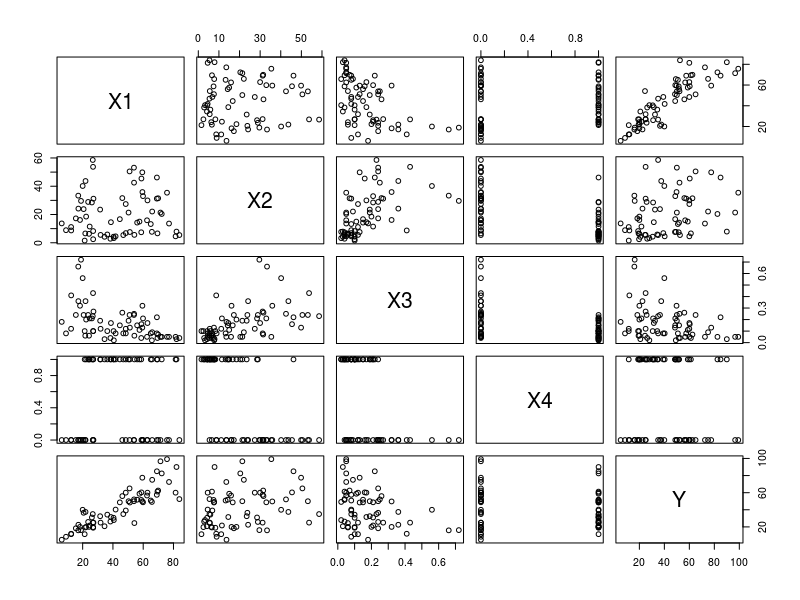
\includegraphics[width=\textwidth]{pairs.png}
\caption{Pairs plot of \texttt{landrent} data.}
\label{fig6}
\end{figure}

We can see that there seems to be a strong linear relation between $Y$ and $X1$. In addition, there seems to be colinearity between $X2$ and $X3$. In order to verify this, we look at the correlation between these two variables (and all the others for good measure) using \texttt{cor}. The correlation matrix is shown in Table \ref{q6}.

\begin{table}[!ht]
\centering
\caption{Correlation matrix for \texttt{landrent} data.}
\begin{tabular}{c|c|c|c|c|c}
    &       Y      &       X1     &       X2      &       X3      &     X4     \\
\hline
 Y  &  1.00000000  &              &               &               &            \\
 X1 &  0.87577226  &  1.00000000  &               &               &            \\
 X2 &  0.30857124  &  0.04871882  &   1.00000000  &               &            \\
 X3 & -0.32337827  & -0.4998227   &   0.5225979   &   1.00000000  &            \\
 X4 & -0.08894927  &  0.08896304  &  -0.58343638  &  -0.08894927  & 1.00000000 \\
\end{tabular}
\label{q6}
\end{table}

 We can see that the correlation between $X2$ and $X3$ is $0.5225979$. In addition, this table shows a correlation between $X2$ and $X4$ as well. These results lead us to believe that $X2$ and $X4$ do not need to be included in the final model.

 We decide to test the model $Y = \beta_0 + \beta_1 X1 + \beta_2 X2$, and get the following results:

 \begin{itemize}
 \item $b_0 = -6.11433$ ($p = 0.043 < 5\%$). This would be the baseline average rent per acre for alfalfa, but does not make sense in this context and can be disregarded.
 \item $b_1 = 0.92137$ ($p < 2 \cdot 10^{-16}$). With the density of dairy cows constant, an increase in rent for all tillable land by one unit leads to and expected increase in the mean rent per acre planted for alfalfa of $0.92137$.
 \item $b_2 = 0.39255$ ($p = 1.59 \cdot 10^{-6}$). With the rent for all tillable land constant, an increase in the density of dairy cows by one unit leads to and expected increase in the mean rent per acre planted for alfalfa of $0.39255$.
 \item The F-test is significant ($F^* = 165.3$ on 2 and 64 degrees of freedom, p-value: $< 2.2 \cdot 10^{-16}$), so there is an overall linear relation between $Y$ and the two regressor variables.
 \item $R^2 = 0.8379$ and $R^2_a = 0.8328$.
 \end{itemize}

 We now make all the necessary tests on the residuals to see if the model is acceptable. All plots are shown in Figure \ref{fig6_2}.

\begin{figure}[!ht]
\begin{subfigure}{.5\textwidth}
  \centering
  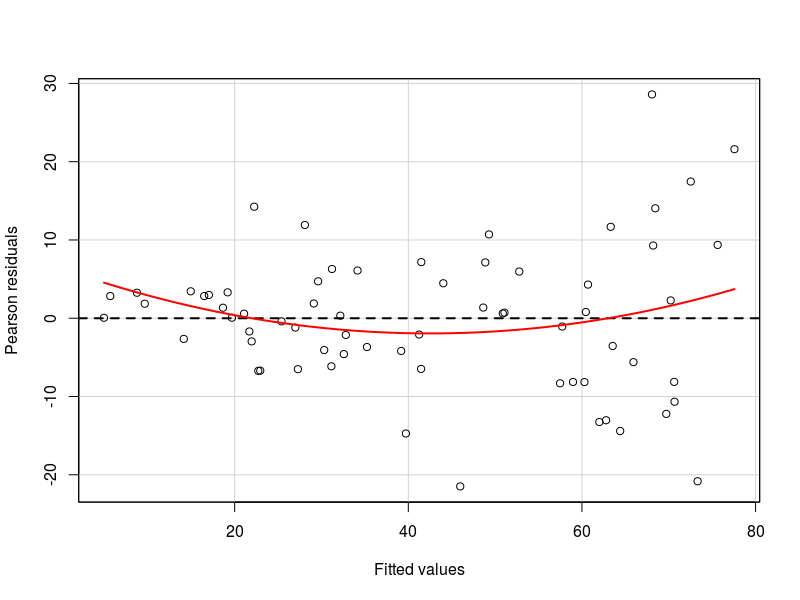
\includegraphics[width=\linewidth]{residPlot6.png}
  \caption{Residual Plot}
  \label{fig6_2:resid}
\end{subfigure}%
\begin{subfigure}{.5\textwidth}
  \centering
  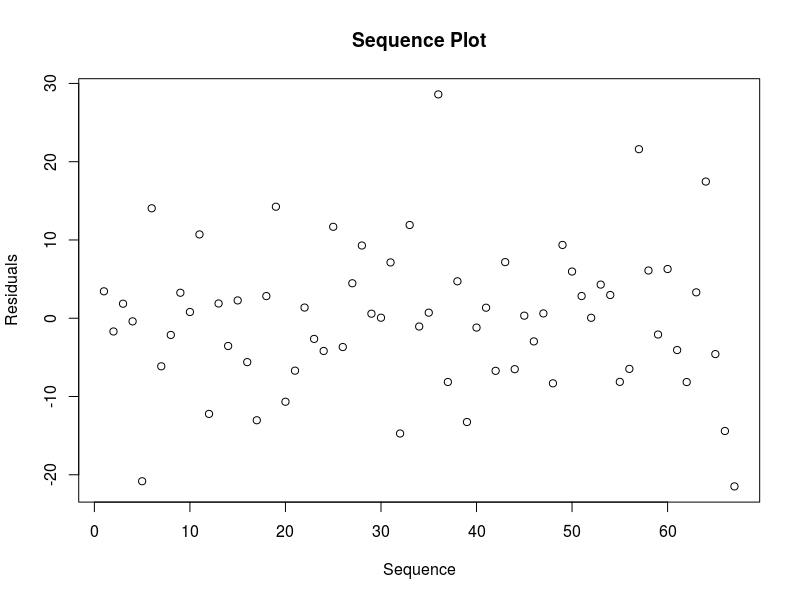
\includegraphics[width=\linewidth]{seqPlot6.png}
  \caption{Sequence Plot}
  \label{fig6_2:seq}
\end{subfigure}
\begin{subfigure}{.5\textwidth}
  \centering
  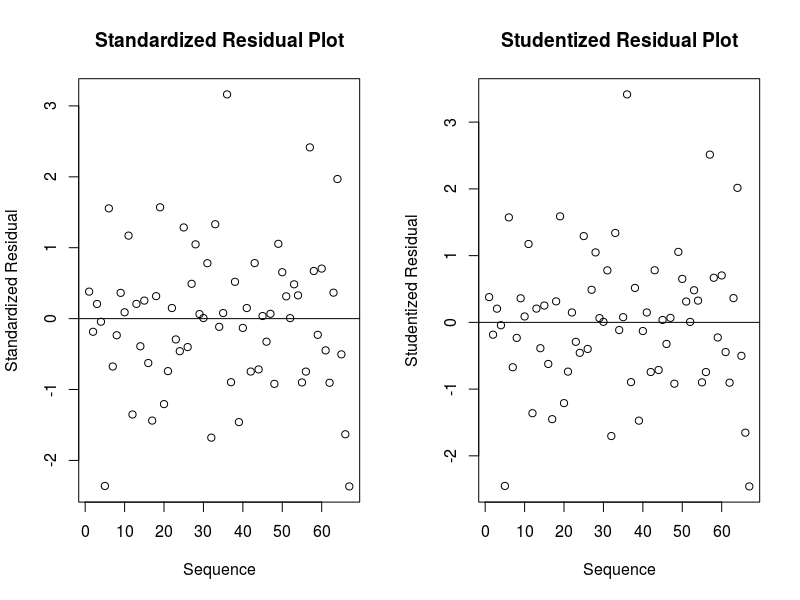
\includegraphics[width=\linewidth]{outliers6.png}
  \caption{Outliers Plot}
  \label{fig6_2:outliers}
\end{subfigure}%
\begin{subfigure}{.5\textwidth}
  \centering
  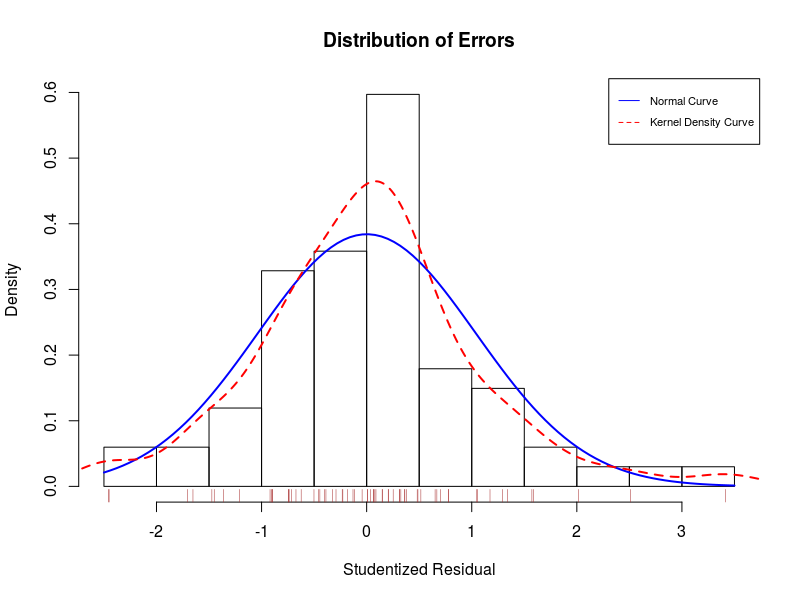
\includegraphics[width=\linewidth]{normality6.png}
  \caption{Normality Plot}
  \label{fig6_2:normal}
\end{subfigure}
\caption{Regression tests for \texttt{landrent} data.}
\label{fig6_2}
\end{figure}

We can see from Subfigure \ref{fig6_2:resid} that the residuals do not seem to be homoskedastic. We use a Brown-Forsythe test in order to determine this. We separate that data into two groups for the variable $X1$ separating along the median value. The p-value obtained this way is $0.07082 > 5\%$, so we do not reject $H_0$ and can say that the residuals are homoskedastic. The sequence plot in Subfigure \ref{fig6_2:seq} shows no sign of dependent residuals. No outliers can be discerned by the Subfigure \ref{fig6_2:outliers}, and the distribution of the residuals seems normal from Subfigure \ref{fig6_2:normal}. This last statement is confirmed by a Shapiro-Wilk test (p-value = $0.3855$) and a QQ-plot (not shown).

We can try to add another variable to the model, to see if it improves the model. If we add $X3$ (for the model $Y = \beta_0 + \beta_1 X1 + \beta_2 X2 + \beta_3 X3$), we get a non-significant estimator for the extra variable. If we add $X4$ (for the model $Y = \beta_0 + \beta_1 X1 + \beta_2 X2 + \beta_3 X4$), we also get a non-significant estimator for the extra variable. In both cases, $R^2_a$ decreases in relation to our first model. The effects of $X3$ and $X4$ are contained in their correlation with $X1$ and $X2$.

In conclusion, we decide to keep the model $Y = \beta_0 + \beta_1 X1 + \beta_2 X2$, for which we have $\hat{Y} = -6.11433 + 0.92137 X1 + 0.39255 X2$. The average rent per acre planted for alfalfa is positively correlated with the average rent paid for all tillable land. In addition, rent for land planted to alfalda relative to rent for other agricultural purposes is higher in areas with high density of dairy cows. However, liming does not have a significant impact of the average price per acre for alfalfa.

\paragraph{\Large Question 7}\normalsize

In this question, two backward stepwise regression algorithms are implemented and tested using the \texttt{Rateprof} dataset. We start by creating the full model, using all predictor variables. Then, one variable is removed at a time, until a criterion is reached. For this exercise, two elimination criterions were implemented:

\begin{itemize}
\item The function \texttt{backstep\_byPvalue} uses a p-value approach in order to determine when to stop removing variables. The $\alpha$ level is defined by the user, with $5\%$ being the default. A variable is removed if the p-value for the significance of its predictor (t-value) is greater than this threshold. The variable with the highest p-value is chosen to be removed. The algorithm stops once all predictors are significant.

\item The function \texttt{backstep\_byAdjR2} uses an $R^2_a$ criterion to justify removing variables. We wish to get the model that gives the highest $R^2_a$. We compare the full model with the one with one less variable in it. If the reduced model has a higher $R^2_a$, then we remove that variable and repeat the process. If the reduced variable has a lower $R^2_a$, it means we have passed the highest return. Therefore, the full model at that step is returned. 
\end{itemize}

Let's call \texttt{lm\_p} and \texttt{lm\_a} the two linear regression models obtained by p-value and ajusted R-squared respectively. We can see from their \texttt{summary} that the linear model with a p-value elimination criteria has only four explanatory variables in the reduced model, whereas the model using an adjusted R-squared criterion had 8 final explanatory variables. If inference is the main objective, the p-value method should be favored. However, the $R^2_a$ for the p-value regression model is $0.9971719$, which is lower than the adjusted R-squared model, for which the $R^2_a$ is $0.9971979$. In this case, the difference between the two does not seem important. For this dataset, the p-value method would be preferable since we have a very high $R^2_a$ with half the predictor variables used (it is more interpretable).

\paragraph{\Large Question 8}\normalsize

See file \texttt{hw4q8.R} for this exercise.

\paragraph{\Large Question 9}\normalsize

See file \texttt{hw4q9.R} for this exercise.

\paragraph{\Large Question 10}\normalsize

In order to test whether Shapiro-Wilk's normality test is reliable, we run a little experiment.

\begin{itemize}
\item First, we explore the robustness of the test for non-normally distributed data when the data set is small ($n = 10$). For this, we run a random uniform distribution between 0 and 1 5000 times. We calculate the percentage of trials that are considered normal by SHapiro-Wilk. In one particular scenario, $91.56\%$ of the trials were mistakenly labeled as normally distributed (since the nature of this test is by definition random, results may vary across experiments). So the Shapiro-Wilk normality test is not powerful for small samples. 
\item Then, we wish to test whether the test is accurate for samples with many data points ($n = 5000$). For this, we use a random standard normal distribution (without any added random noise). In my run, I got $4.16\%$ of the trials that were considered non-normally distributed. The data points were picked from the same \textbf{normal} distirbution, and yet more than $4\%$ of the trials were not considered normal by Shapiro-Wilk's normality test. So it is too powerful when the sample size is large.
\end{itemize}

This empirical example shows that Shapiro-Wilk's test by itself is not a good measure of a sample's normality. It can be used as a starting point for analysis, but other tests (either visual such as a QQ-plot) or quantitative (such as a test for skweness for example).

\end{document}